\chapter{Appendix}
The appendix contains diagrams and tables that were to big to put them into the continuous text. Furthermore, it contains a small installation manual for the \ac{HiP} backend.

\section{Installation manual}
The installation process of the \ac{HiP} backend is quite simple. In general, you need to install 3 different things: The Play 2.0 framework, the MongoDB and \ac{NPM}. In more detail, the process looks like this:

\begin{enumerate}
	\item Get your Play 2.0 framework instance from \url{https://www.playframework.com/download}
	\item Install Play 2.0 (do NOT run it at this point in time)
	\item Go to your \ac{HiP} root folder
	\item Switch to \%hipRoot/public
	\item Run npm link on your command line
	\item Download MongoDB from \url{http://www.mongodb.org/downloads}
	\item Run the MongoDB with the provided default database (this can be done on a Windows PC with the following command: \\ \verb|mongod --dbpath $<<$PATH TO THE PROVIDED DB$>>$)|
	\item Again: Go to your \ac{HiP} root folder
	\item	Start the \ac{HiP} backend by using the command: activator run
\end{enumerate}

Your \ac{HiP} server is now running. After you have installed all the needed components you can easily run the test cases for the controllers with the following commands:

\begin{enumerate}
	\item Switch to \%hipRoot/public
	\item	Start the \ac{HiP} test cases by using the command: karma start karma.conf
\end{enumerate}

After we have now seen how we can start the application and the provided test cases, the remaining part of the appendix will contain bigger figures and tables.

\section{Figures and tables}
Figure \ref{workflow_backend} shows the work-flow within the backend system as a flow diagram.

\begin{figure}[ht]
\centerline{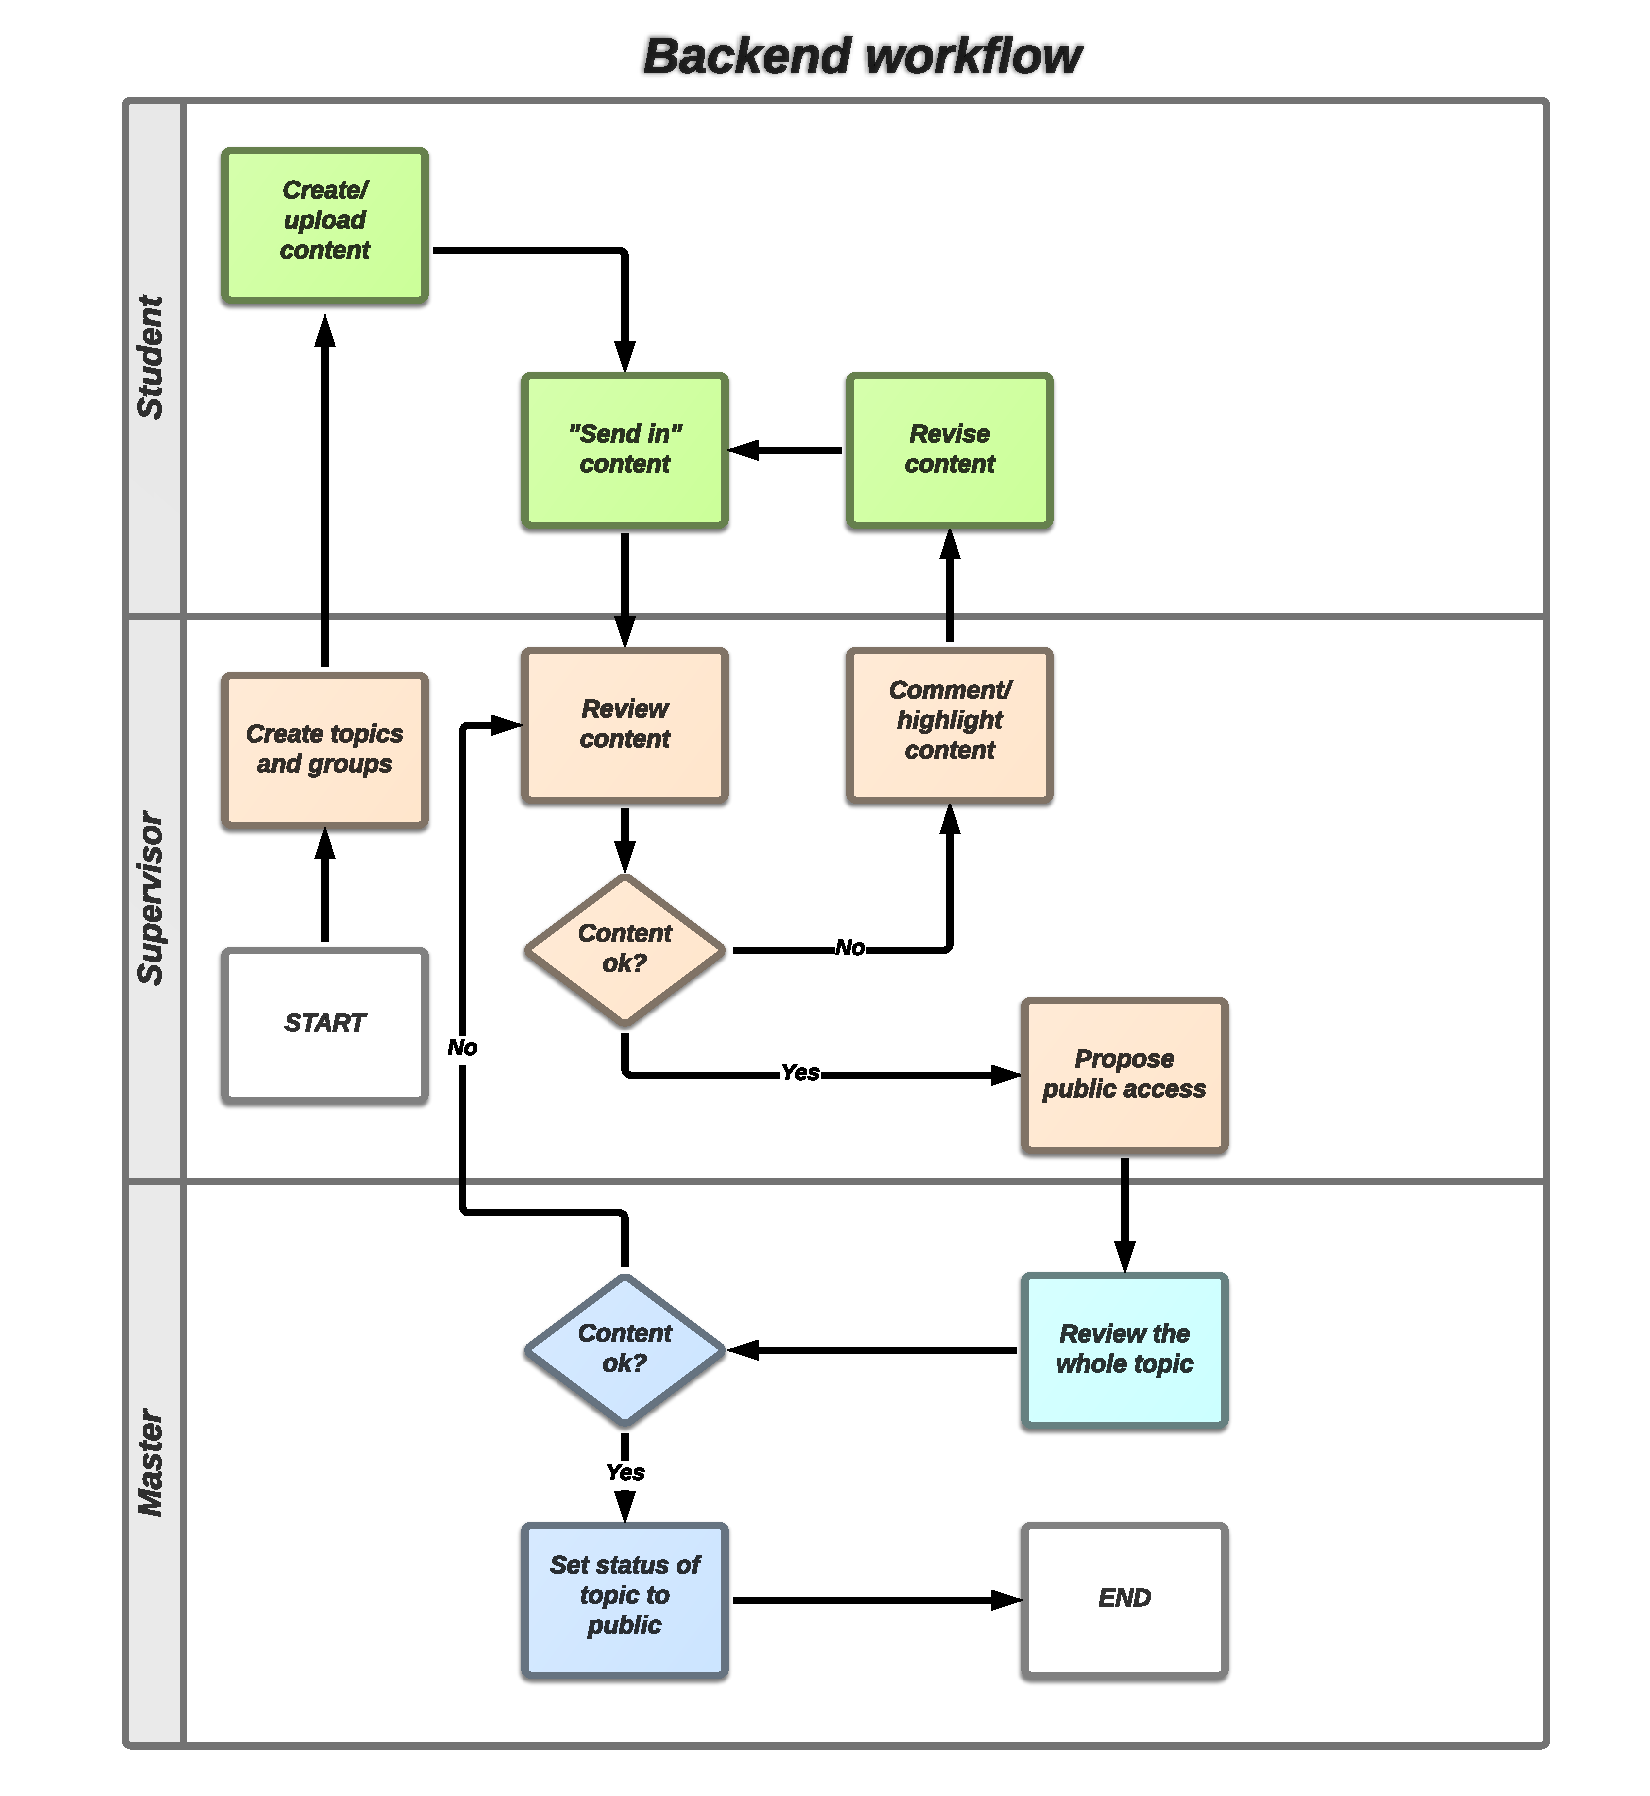
\includegraphics[width=1.3\textwidth]{gfx/HiP-Backend-Workflow}}
\caption{The diagram shows the work-flow within the backend system with the three roles that are involved in the work-flow.}
\label{workflow_backend}
\end{figure}

Furthermore, Figure \ref{usecase} shows an \ac{UML2} use case diagram showing the different users (i.e., user roles) of the application and Figure \ref{UML:deploymentDiagram} shows a more technical view on the deployment situation of the system.

\begin{figure}[ht]
\centerline{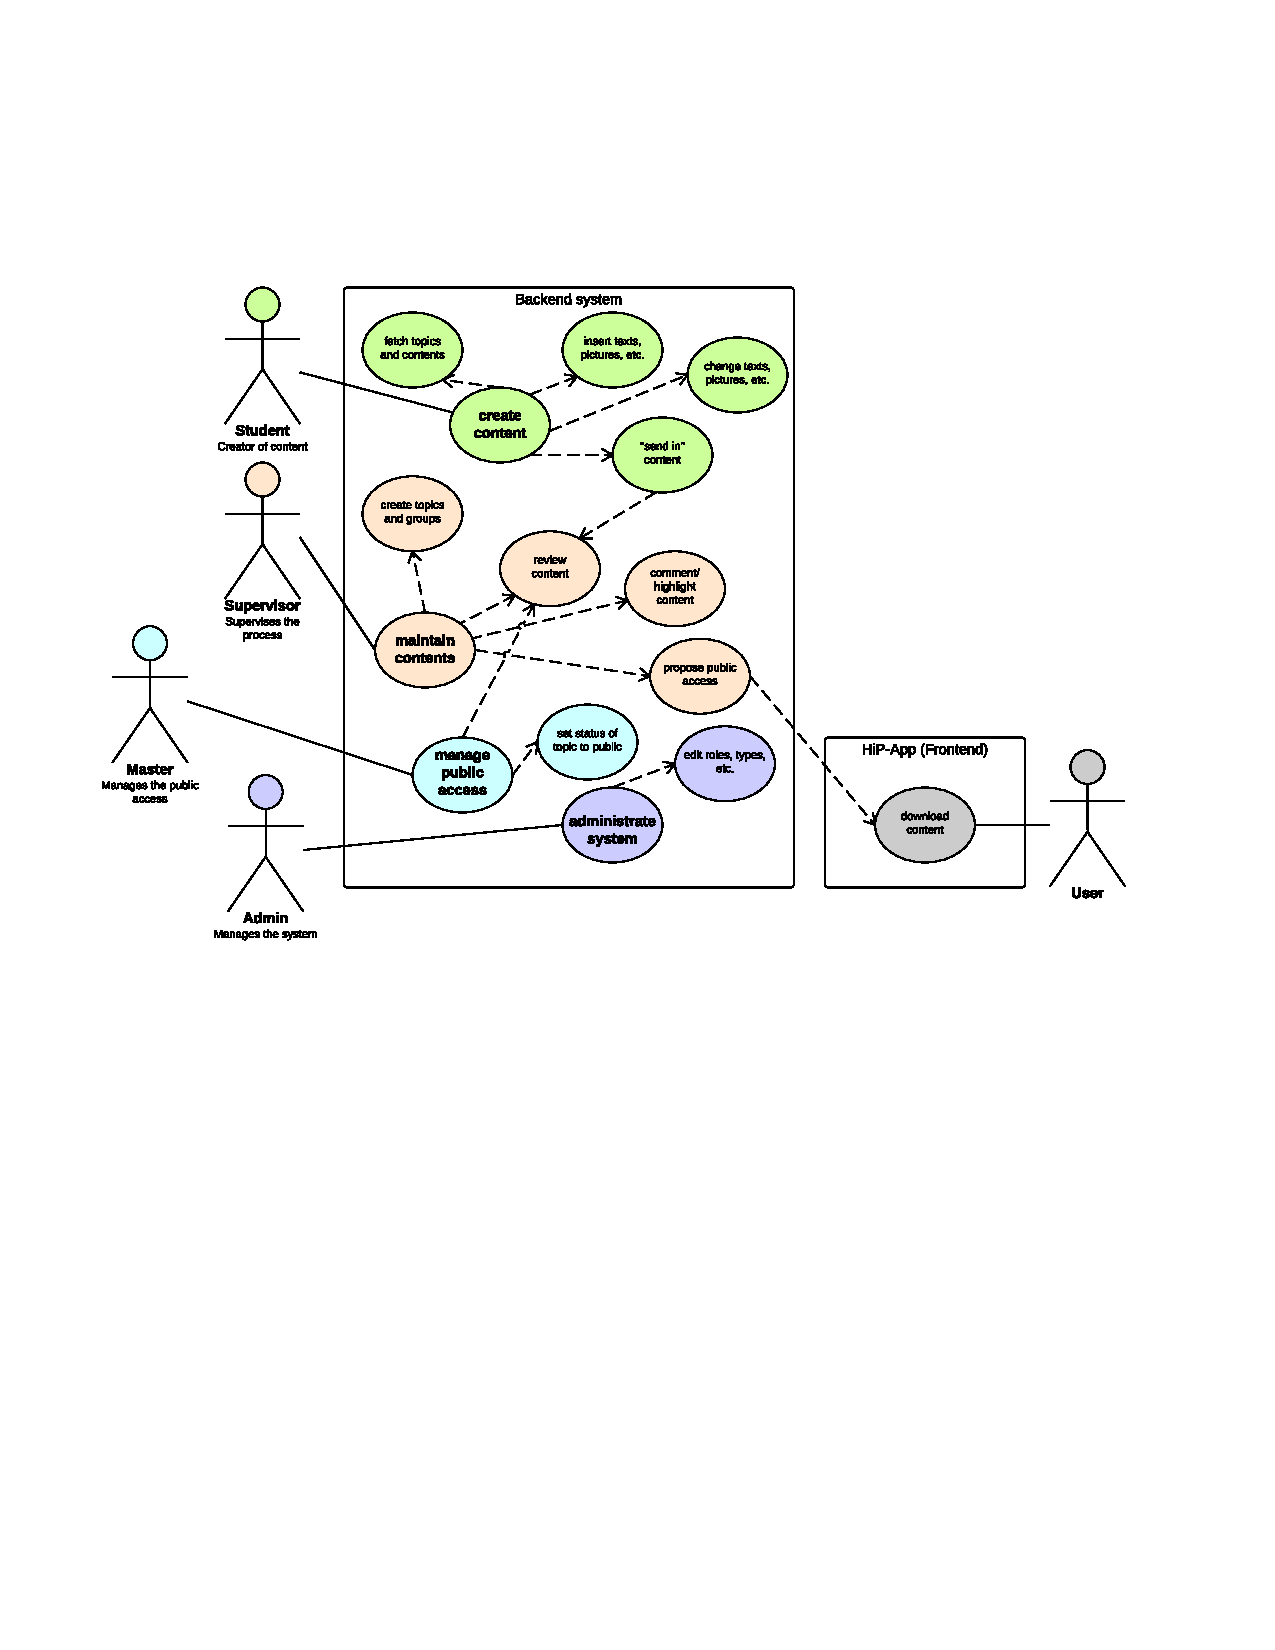
\includegraphics[width=1.4\textwidth]{gfx/HiP-UseCase_Diagramm}}
\caption{An \ac{UML2} use case diagram showing the different users of the \ac{HiP} system.}
\label{usecase}
\end{figure}

\begin{figure}[ht]
\centerline{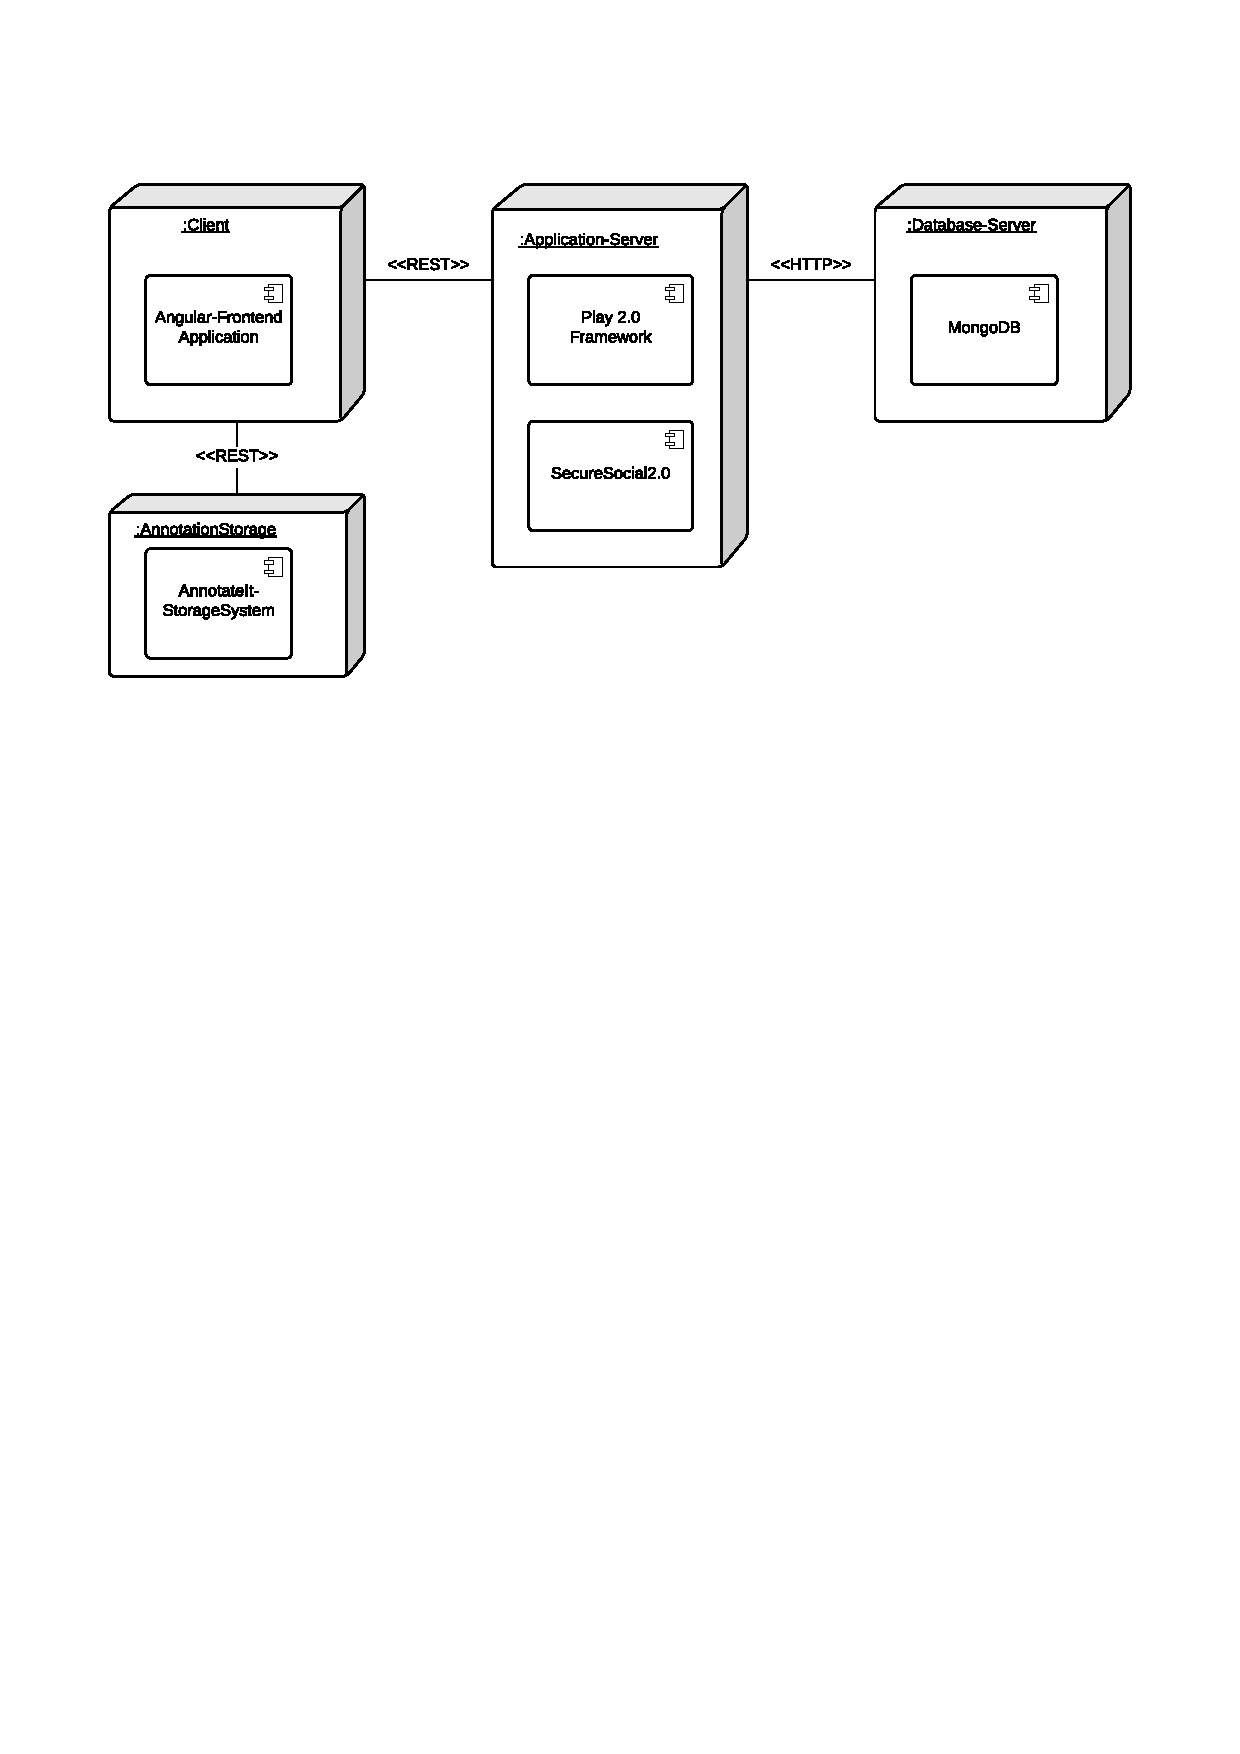
\includegraphics[width=1.3\textwidth]{gfx/HiPDeployment}}
\caption{An \ac{UML} deployment diagram showing the different parts of the \ac{HiP} application.}
\label{UML:deploymentDiagram}
\end{figure}

The IDs of the entries within the tables, which are written in bold letters, will be done within the master-thesis itself. The remaining parts may be done via, for example, project-groups, etc. 

\afterpage{%
    \clearpage% Flush earlier floats (otherwise order might not be correct)
    \thispagestyle{empty}% empty page style (?)
    \begin{landscape}% Landscape page
        \centering % Center table
	\begin{center}
	
\begin{longtable}{|l|l|lll|}
\caption{Showing the derived requirements of the backend for the supervisor role, which are sorted by priority.} 
\label{RequirementsBackendSupervisor} \\

\hline 
	\multicolumn{1}{|c|}{\textbf{ID}} & \multicolumn{1}{c|}{\textbf{Description}} & \multicolumn{1}{c|}{\textbf{Acceptance criteria}} & \multicolumn{1}{c|}{\textbf{Priority}} \\ \hline 
\endfirsthead

\multicolumn{3}{c}%
{{\bfseries \tablename\ \thetable{} -- continued from previous page}} \\
\hline 	\multicolumn{1}{|c|}{\textbf{ID}} & \multicolumn{1}{c|}{\textbf{Description}} & \multicolumn{1}{c|}{\textbf{Acceptance criteria}} & \multicolumn{1}{c|}{\textbf{Priority}} \\ \hline 
\endhead

\hline \multicolumn{3}{|r|}{{Continued on next page}} \\ \hline
\endfoot

\hline \hline
\endlastfoot
		\hline
	\textbf{BS1} 	& The supervisor should draft \textbf{guidelines} 		& - At least one information resp. help 	& 1	\\
	 		& and assistance (e.g., Button with question-mark)		& function per functionality 			& 		\\
	\hline
	\textbf{BS2} 	& The supervisor should be able to see 				&  - The feedback should be visual	& 1	\\
	 	& \textbf{which data is missing} 					&  - The feedback should be transparent to	& 	\\
		& 											& upper layers of the UI & \\
	\hline
	\textbf{BS3} 	& The supervisor should be able to see 				& - Try without content that is ready & 1\\
	 	& \textbf{data that is ready} for review 				&  for review & \\
		&											& - Try with content that is ready		& \\
		&											& for review		& \\
	\hline
	\textbf{BS4} 	& The supervisor should be able to \textbf{assign} 	& - Try assigning an exhibit to one & 1\\
	 	& \textbf{exhibits} to students 					& student  & \\
		&										& - Try assigning an exhibit to more	& \\
		&										&	than one student				& \\
	\hline
	\textbf{BS5} 	& The supervisor should be able to \textbf{trace} 		& - Show visual connection between	& 1\\
	 	& \textbf{content} back to specific students 			&  student and content 	& \\
	\hline
	\textbf{BS6} 	& The supervisor should be able to \textbf{define}  	&  - Try defining a topic more than once	& 1\\
	 	& \textbf{topics} and exhibits  				    		&  	& \\
	\hline
	\textbf{BS7} 	& The supervisor should be able to \textbf{comment} 		& - Try commenting empty content		& 1\\
		& \textbf{and discuss} the given content of the students 	&- Try commenting a lot of content		& \\	
	\hline
	\textbf{BS8} 	& The supervisor should be able to \textbf{mark} 	& - Try marking an error twice & 1\\
		& \textbf{errors} in the content					&	& \\
	\hline
	BS9 	& The supervisor should get \textbf{e-mail notifications} 	& - The message should leave the system  & 1\\
		& about new content handed in by students		& in less than 2 minutes in 90\% of the time	& \\
	\hline
	\textbf{BS10}& The supervisor should be able to \textbf{copy topics} 		& - Try copy an empty topic  		& 2\\
		& and categories (e.g., usage of templates				& - The copied topic should be easily		&		\\
		& for different typical cases, duplication, etc.)				& changeable to adapt it to the new usage		& \\
	\hline
	\textbf{BS11}& The supervisor should be able to define 				& - Try with error within the validation & 2\\
		& \textbf{validation-constraints} (e.g., character			& constraints & \\
		& limitation)										& 			& \\
	\hline
	\textbf{BS12}& The supervisor is able to see the \textbf{amount}		& - Try without any content included & 2\\
		& of \textbf{texts and pictures} in a hidden topic			& - Try with a lot of content included	& \\
	\hline
	BS13& The supervisor should be able to \textbf{work offline} 	& - Try disconnecting a running session & 3\\
\end{longtable}
\end{center} 
    \end{landscape}
    \clearpage% Flush page
}

\afterpage{%
    \clearpage% Flush earlier floats (otherwise order might not be correct)
    \thispagestyle{empty}% empty page style (?)
    \begin{landscape}% Landscape page
        \centering % Center table
	\begin{center}
	
\begin{longtable}{|l|l|lll|}
\caption{Showing the derived requirements of the Backend for the student role, which are sorted by priority.} 
\label{RequirementsBackendStudent} \\

\hline 
	\multicolumn{1}{|c|}{\textbf{ID}} & \multicolumn{1}{c|}{\textbf{Description}} & \multicolumn{1}{c|}{\textbf{Acceptance criteria}} & \multicolumn{1}{c|}{\textbf{Priority}} \\ \hline 
\endfirsthead

\multicolumn{3}{c}%
{{\bfseries \tablename\ \thetable{} -- continued from previous page}} \\
\hline 	\multicolumn{1}{|c|}{\textbf{ID}} & \multicolumn{1}{c|}{\textbf{Description}} & \multicolumn{1}{c|}{\textbf{Acceptance criteria}} & \multicolumn{1}{c|}{\textbf{Priority}} \\ \hline 
\endhead

\hline \multicolumn{3}{|r|}{{Continued on next page}} \\ \hline
\endfoot

\hline \hline
\endlastfoot
		\hline
	\textbf{BSt1} & The students are only able to \textbf{send in} 		& - Try sending content to another topic & 1	\\
	 	& \textbf{specific content} (field / topic) 				&  & 		\\
	\hline
	BSt2	& The students should get an \textbf{e-mail noti-} 	& - The e-mail should be received in less & 1	\\
	 	& \textbf{fiation} about new content in their topic 	& than 2 minutes in 90\% of the time & 	\\
	 	& (e.g., send in via fellow students) 			&  & 	\\
	\hline
	\textbf{BSt3} & The students should be able to send in  		& - Try with errors within the meta-data & 1\\
	 	& \textbf{metadata} 							&  & \\
	\hline
	\textbf{BSt4} & The students should be able to \textbf{overview} 	& - Try without any links & 1\\
	 	& the \textbf{possible links} within their topic 			& - Try with a lot of links & \\
	 	& (e.g., GPS-information) 						&  & \\
	\hline
	\textbf{BSt5} & The students should be able to \textbf{send in}  		& - Try sending empty content  & 1\\
	 	& \textbf{content}								& - Try sending a lot of content  & \\
	\hline
	\textbf{BSt6} & The students should be able to \textbf{propose}  	& - Try proposing an existing topic  & 1\\
	 	& topics and content  				    			&  & \\
	\hline
	BSt7 & The students should only have \textbf{access}  		& - Try logging in after the temporary & 1\\
		& to the backend \textbf{for a specific time} 			& account has been deleted	& \\	
	\hline
	\textbf{BSt8} & The students should have \textbf{access to all} 		& - Try accessing currently empty content  	& 1\\
		& temporary content (i.e., not reviewed 				&	& \\
		&	content)									&	& \\
	\hline
	\textbf{BSt9} & The students should be able to create 			& - Try creating a group without users  	& 1\\
		& \textbf{interdisciplinary groups} and communicate	& - Try to send an empty message to	& \\
		& within these									& the group	& \\
		& 											& - Try to send a very long message to	& \\
		& 											& the group	& \\
	\hline
	BSt10& The students should be able to see their 			& - Try showing an empty topic 	& 2\\
		& content in a \textbf{preview mode} that simulates	& - Try showing a huge topic	&	\\
		& the frontend									&	& \\
	\hline
	BSt11& The students should be able to see content 		& -  Try showing an empty topic & 2\\
		& of \textbf{other groups in a preview} mode that 		& - Try showing a huge topic	&	\\
		& simulates the frontend							&	& \\
	\hline
	\textbf{BSt12}& The students should be able to comment  			& - Try to send an empty comment  & 2\\
		& and \textbf{discuss} the content of their group		& - Try to send a huge comment	 & \\
		& or other groups								&	 & \\
	\hline
	\textbf{BSt13}& The students should be able to \textbf{hide} their 	& - Try hiding without having any content & 2\\
		& unfinished work to the supervisor					&	& \\
\end{longtable}
\end{center} 
    \end{landscape}
    \clearpage% Flush page
}

\afterpage{%
    \clearpage% Flush earlier floats (otherwise order might not be correct)
    \thispagestyle{empty}% empty page style (?)
    \begin{landscape}% Landscape page
        \centering % Center table
	\begin{center}
	
\begin{longtable}{|l|l|lll|}
\caption{Showing the derived requirements of the Backend for the master role, which are sorted by priority.} 
\label{RequirementsBackendMaster} \\

\hline 
	\multicolumn{1}{|c|}{\textbf{ID}} & \multicolumn{1}{c|}{\textbf{Description}} & \multicolumn{1}{c|}{\textbf{Acceptance criteria}} & \multicolumn{1}{c|}{\textbf{Priority}} \\ \hline 
\endfirsthead

\multicolumn{3}{c}%
{{\bfseries \tablename\ \thetable{} -- continued from previous page}} \\
\hline 	\multicolumn{1}{|c|}{\textbf{ID}} & \multicolumn{1}{c|}{\textbf{Description}} & \multicolumn{1}{c|}{\textbf{Acceptance criteria}} & \multicolumn{1}{c|}{\textbf{Priority}} \\ \hline 
\endhead

\hline \multicolumn{3}{|r|}{{Continued on next page}} \\ \hline
\endfoot

\hline \hline
\endlastfoot
		\hline
	BM1 & The master should be able to \textbf{recover data} 	& - The recovery should not take & 1	\\
	 	& by using a back-up system					& longer than one hour & 		\\
	\hline
	\textbf{BM2} & The master role can be assigned to 				& - Try to assign the master role to nobody & 2	\\
	 	& a \textbf{couple of users} at the same time 			&  & 	\\
	\hline
	\textbf{BM3} & The master is able to do the final  				& - Try to accept an empty topic & 2\\
	 	& \textbf{acceptance} 							& - Try to accept a huge topic & \\
\end{longtable}
\end{center} 
    \end{landscape}
    \clearpage% Flush page
}

\afterpage{%
    \clearpage% Flush earlier floats (otherwise order might not be correct)
    \thispagestyle{empty}% empty page style (?)
    \begin{landscape}% Landscape page
        \centering % Center table
	\begin{center}
	
\begin{longtable}{|l|l|lll|}
\caption{Showing the derived requirements of the Backend, which are sorted by priority.} 
\label{RequirementsBackendMisc} \\

\hline 
	\multicolumn{1}{|c|}{\textbf{ID}} & \multicolumn{1}{c|}{\textbf{Description}} & \multicolumn{1}{c|}{\textbf{Acceptance criteria}} & \multicolumn{1}{c|}{\textbf{Priority}} \\ \hline 
\endfirsthead

\multicolumn{3}{c}%
{{\bfseries \tablename\ \thetable{} -- continued from previous page}} \\
\hline 	\multicolumn{1}{|c|}{\textbf{ID}} & \multicolumn{1}{c|}{\textbf{Description}} & \multicolumn{1}{c|}{\textbf{Acceptance criteria}} & \multicolumn{1}{c|}{\textbf{Priority}} \\ \hline 
\endhead

\hline \multicolumn{3}{|r|}{{Continued on next page}} \\ \hline
\endfoot

\hline \hline
\endlastfoot
		\hline
	BMi1 & The data of the system is \textbf{stored} on IMT- 		& - The data should be easily transferable & 1	\\
	 	& Server											&  	& 		\\
	\hline
	\textbf{BMi2} & The system can be \textbf{updated} and  		&  	& 1	\\
	 	& maintained in the future							&  	& 	\\
		& (e.g., project-groups, SHK, etc.)						& 	& \\
	\hline
	\textbf{BMi3} & The content should not be limited to				&  	& 1\\
	 	& specific \textbf{layouts, views} (e.g., languages)			&	& \\
		& and templates 									&  	& \\
		\hline
	\textbf{BMi4} & The system should be \textbf{expandable} 		&  	& 1	\\
	 	& (e.g., new content, filters, etc.)						&  	& 		\\
	\hline
	\textbf{BMi5} & The system should be \textbf{safe} with respect 	& -The system should be safe with 	& 1	\\
	 	& to hackers resp. data manipulation 					&  respect to the economic view/ 	& 	\\
		&												& definition of safety			&\\
	\hline
	\textbf{BMi6} & The system offers features to \textbf{manage}  	& - Try managing a group with an empty name  & 2\\
	 	& groups 											& 	 & \\
\end{longtable}
\end{center} 
    \end{landscape}
    \clearpage% Flush page
}

\afterpage{%
    \clearpage% Flush earlier floats (otherwise order might not be correct)
    \thispagestyle{empty}% empty page style (?)
    \begin{landscape}% Landscape page
        \centering % Center table
	\begin{center}
	
\begin{longtable}{|l|l|lll|}
\caption{Showing the derived requirements of the Frontend, which are sorted by priority.} 
\label{RequirementsFrontend} \\

\hline 
	\multicolumn{1}{|c|}{\textbf{ID}} & \multicolumn{1}{c|}{\textbf{Description}} & \multicolumn{1}{c|}{\textbf{Acceptance criteria}} & \multicolumn{1}{c|}{\textbf{Priority}} \\ \hline 
\endfirsthead

\multicolumn{3}{c}%
{{\bfseries \tablename\ \thetable{} -- continued from previous page}} \\
\hline 	\multicolumn{1}{|c|}{\textbf{ID}} & \multicolumn{1}{c|}{\textbf{Description}} & \multicolumn{1}{c|}{\textbf{Acceptance criteria}} & \multicolumn{1}{c|}{\textbf{Priority}} \\ \hline 
\endhead

\hline \multicolumn{3}{|r|}{{Continued on next page}} \\ \hline
\endfoot

\hline \hline
\endlastfoot
		\hline
F1 & The user should be able to \textbf{navigate} 			&  - The navigation should response fast  		& 1\\
	 	& to the different locations shown in the 				&  - Try navigating to the current position		& \\
		& HiP-application 								&		&	\\
	\hline
	F1.A & The user should be able to navigate 				&  See F1		& 1\\
	 	& to the different locations and discover 				&  		& \\
		& these locations on his own 						&		&	\\
	\hline
	F1.B & The user should be able to navigate 				&  See F1		& 1\\
	 	& to the different locations and use 				&  		& \\
		& round tour information of the application 			&		&	\\
		\hline
	F1.B & The user should be able to navigate 				& See F1	 	& 1\\
	 	& to the different locations while using  				&  		& \\
		& filters (e.g., epochs)							&		&	\\
	\hline
	F2 & The user should be able to create \textbf{thematic} 	& - Try creating a route without assigning & 1\\
		& \textbf{routes} 								& a theme & \\
	\hline
	F3 & The user should get a \textbf{list of locations/exhibits} 	& - Try opening an empty list  	& 1\\
		& in Paderborn									&	& \\
	\hline
	F4 & The user should \textbf{see linkings} within an exhibit  	&  - Try opening a topic without links	& 1\\
		& different exhibits (e.g., Liborischrein -> Hle ->		& - Try opening a topic with a lot of links	& \\
		& Scriptorium) 									&	& \\
	\hline
	F5 & The user should be able to \textbf{deselect} specific 	& - Try deselect only one & 1\\
		& categories 									& - Try deselect many	& \\
	\hline
	F6 & The user should be able to \textbf{filter} exhibits on  	& - Try using multiple filters  	& 1\\
		& the map (e.g., locations, historical figures, 			&	& \\
		& etc.)										&	& \\
	\hline
	F7 & The user is able to \textbf{overlay} the current map  	& - Try overlay one map with a hist. one & 1\\
		& of the city with historical maps					& - Try overlay a couple of maps	& \\
	\hline
	F8 & The user is able to \textbf{see himself and historical} 	& - Try in an area without hist. places  	& 1\\
		& places on the map 							& - Try in an area with a lot of hist. places	&  \\
	\hline
	F9 & The user should not \textbf{exceed his storage} 		& - Clear cache should be possible  	& 1\\
		& on the smartphone							&	& \\
	\hline
	F10 & The user should not \textbf{exceed his data-volume} 	& - Pictures and videos have to be   	& 1\\
		& on the smartphone							& small	& \\
	\hline
	F11 & The user should be able to use the  				&  - Interface should not include too many 	& 1\\
		& application easily (\textbf{good usability})			& functions per view 	& \\
		F12 & The user should be able to switch between 			& - At most two clicks/touches between  	& 1\\
		& \textbf{different contents} (e.g., Video, 3D, etc.)		& the different contents	& \\
		& fast										&	& \\
	\hline
	F13 & The user should be able to see \textbf{\textit{invisible}} 	& - Try with more than one invisible 	& 1\\
		& objects within the details-tab (e.g., something			& object at the same time	& \\
		& placed inside an altar)								&	& \\
	\hline
	F14 & The user should be able to use \textbf{tablets} and 		& - The UI should adapt to the screen size  	& 1\\
		& smartphones									& resp. resolution	& \\
	\hline
	F15 & The user should only get details about an  				& - Try to get details beforehand & 1\\
		& exhibit while he is \textbf{next to it or afterwards} 		&	& \\
	\hline
	F16 & The user should be able to get \textbf{texts, graphics/}  	& - Try without any texts, etc.  & 1\\
		& \textbf{pictures} and links about an exhibit				& - Try with a lot of texts, etc.  	& \\
	\hline
	F17 & The user should be able to get \textbf{audio, video}  		& - Try without any videos, etc.    & 2\\
		& and \textbf{3D-views/models} about an exhibit			& - Try with a lot of videos, etc.  	& \\
	\hline
	F18 & The user can create and join \textbf{treasure hunts} 		& - Try join an treasure hunt without a name & 2\\
		& respectively geo-caching features					&	& \\
	\hline
	F19 & The user should get informed about \textbf{exhibits} 		& - The information should be send immediately  & 2\\
		& and \textbf{locations that are next to him}				& as the user arrives at the position		& \\
	\hline
	F20 & The user should be able to get navigated 				& See F1  & 2\\
		& with \textbf{AR-rabbits} 							&		& \\
	\hline
	F21 & The user should be able to get navigated  				& - The navigation should be accurate   & 2\\
		& inside of a \textbf{building}							&	& \\
	\hline
	F22 & The user should be able to choose between 			&    & 2\\
		& different \textbf{starting possibilities} (i.e., tour, 			&	& \\
		& discovery and historical topics) 						&	& \\
	\hline
	F23 & The user should be able to \textbf{hear the content} 		& - The audio files should be small  & 2\\
		& via an audio-guide								& (see, F9, F10)	& \\
	\hline
	F24 & The user should be able to get exhibits as 				&  - Try opening more than one exhibit as& 2\\
		& \textbf{comparison by using AR}						& comparison	& \\ 
	\hline
	F25 & The user should be able to \textbf{create own} 			& - Try creating an empty note/comment  & 2\\
		& \textbf{notes and comments}						& - Try creating a huge note/comment	& \\
	\hline
	F26 & The user should be able to \textbf{share content} 		& - Sharing should not need more than two clicks & 2\\
		& via social media									&		& \\
	\hline
	F27 & The user should be able to \textbf{export content} 		& - The export should not take longer than  & 2\\
		& as PDF and create book-marks						& 30 sec in 90\% of the time	& \\
	\hline
	F28 & The user should be able to get the content 				& - Adding new languages should be easy  & 2\\
		& in \textbf{different languages} (i.e., english, french, 		&	& \\
		& turkish) 										&	& \\
	\hline
	F29 & The user should be able to choose between  			& - Try selecting one criterion & 2\\
		& different \textbf{criteria} with respect to the audience 		& - Try selecting more than one criterion	& \\
		& (e.g., different ages of people) 						&	& \\
\end{longtable}
\end{center} 
    \end{landscape}
    \clearpage% Flush page
}

\afterpage{%
    \clearpage% Flush earlier floats (otherwise order might not be correct)
    %\thispagestyle{empty}% empty page style (?)
    \begin{landscape}% Landscape page
        \centering % Center table
	\begin{center}
	
\begin{longtable}{|l|l|lll|}
\caption{The found usability problems within the walktrough.} 
\label{UsabilityProblems} \\

\hline 
	\multicolumn{1}{|c|}{\textbf{ID}} & \multicolumn{1}{c|}{\textbf{Description}} & \multicolumn{1}{c|}{\textbf{Solved within last version}} & \multicolumn{1}{c|}{\textbf{Priority}} \\ \hline 
\endfirsthead

\multicolumn{3}{c}%
{{\bfseries \tablename\ \thetable{} -- continued from previous page}} \\
\hline 	\multicolumn{1}{|c|}{\textbf{ID}} & \multicolumn{1}{c|}{\textbf{Description}} & \multicolumn{1}{c|}{\textbf{Solved within last version}} & \multicolumn{1}{c|}{\textbf{Priority}} \\ \hline 
\endhead

\hline \multicolumn{3}{|r|}{{Continued on next page}} \\ \hline
\endfoot

\hline \hline
\endlastfoot
		\hline
	UW01 & Use better icons (e.g., flaticons.com) & Yes & 1 \\
	UW02 & Make tabs better recognizable & Yes & 1 \\
	UW03 & Use <a> with href to force other mouse cursor & Yes & 1 \\
	UW04 & Create a new way to show topics/subtopics & No & 1 \\
	UW05 & Be able to include group members to existing groups & Yes & 1 \\
	UW06 & Include imprint & Yes & 1 \\
	UW07 & Startpage: Use a better position to the login button & Yes & 1 \\
	UW08 & Startpage: Describe system better & Yes & 1 \\
	UW09 & Groups: Exchange \emph{Welcome to the group}  & Yes & 1 \\
	UW10 & Groups: Request confirmation on delete & Yes & 1 \\
	UW11 & Groups: Use light signs to show status & Yes & 1 \\
	UW12 & Groups: Show content as tree-structures & No & 1 \\
	UW13 & Groups: Add user-feedback to the dialogue & Yes & 1 \\
	UW14 & Chat: Improve the whole chat system (i.e., make it global) & No & 1 \\
	UW15 & Topic creation: Add free-text search  & Yes & 1 \\
	UW16 & Topic creation: Show subtopics in tree-structures  & No & 1 \\
	UW17 & Topic creation: Add status \emph{hidden}  & Yes & 2 \\
	UW18 & Topic modification: Use groups as first filter  & No & 1 \\
	UW19 & Group creation: Show subtopics in tree-structures  & No & 1 \\
	UW20 & Group creation: Use simpler date-picker  & No & 2 \\
	UW21 & Group-box: Remove refresh button  & Yes & 2 \\
	UW22 & Template-box: Do not close menu by clicking on the \emph{<div>}  & Yes & 2 \\
	UW23 & Template-box: Exchange the way the pulldown-button works  & Yes & 2 \\
	UW24 & Template-box: Use a scroll-view for the preview mode  & No & 3 \\
	UW25 & Browse: Remove button  & Yes & 3 \\
	UW26 & Notification-box: Exchange icon for filter  & Yes & 2 \\
	UW26 & Notification-box: Show data more tabular  & No & 2 \\
	UW27 & Navigation: Remove Home-button  & Yes & 2 \\
	UW28 & Navigation: Show the currently logged-in user  & Yes & 2 \\
	UW29 & Mail-system: Show user-feedback for sent-messages & Yes & 2 \\
	UW30 & Mail-system: Add outbox  & Yes & 2 \\	
	UW31 & Mail-system: Show usernames and not mail-addresses  & Yes & 2 \\
	UW32 & Mail-system: Add e-mail notification for in-system messages  & No & 2 \\
	UW33 & Contact form: Add contact form  & No & 3 \\
	UW34 & Propose topics: More help-text & Yes & 2 \\
	UW35 & Propose topics: Wrong label on button  & Yes & 2 \\
	UW36 & Topic edit: Exchange full-screen logo  & Yes & 3 \\
	UW37 & Topic edit: Edit-frame is buggy  & No & 3 \\
	UW38 & Topic edit: Automatically show new pictures  & Yes & 2 \\
	UW39 & Topic edit: Exchange editor-plugin  & No & 3 \\
	UW40 & Topic edit: Do not switch view on map by click on the map  & Yes & 2 \\
	UW41 & Topic edit: Make Button labels better understandable  & No & 2 \\
	UW42 & Topic edit: Show what is located at a given GPS position & No & 2 \\
	UW43 & Topic edit: Add autocomplete for address field (GPS) & No & 2 \\
	UW44 & Topic edit: Change position of footnote-box with respect  & Yes & 2 \\
	& to locality  &  &  \\
	UW45 & Topic edit: Do not use red-colors on buttons & Yes & 2 \\
	UW46 & Topic edit: Add delete-mode for tags to prevent deleting & Yes & 2 \\
	& by accident   &  &  \\
	UW47 & Topic edit: Order of history is buggy  & No & 2 \\
\end{longtable}
\end{center} 
    \end{landscape}
    \clearpage% Flush page
}

\clearpage

\lstset{language=JavaScript,
basicstyle=\small,
showspaces=false,
showstringspaces=false,   
tabsize=2,
backgroundcolor=\color{grey}}
\begin{lstlisting}[numbers=left,caption={Complete upload Action of the FileController},label=Scala:Upload:full,frame=tlbr,breaklines]
def upload(topicID: String) = Action(parse.multipartFormData) { request =>
    request.body.file("file") match {
      case Some(photo) =>
        val TARGET_W = 64; // width of the thumbnail
        val TARGET_H = 64; // height of the thumbnail

        val filename = photo.filename
        val contentType = photo.contentType

        val newFile = new File("/tmp/picture/uploaded")

        if (newFile.exists())
          newFile.delete()

        photo.ref.moveTo(newFile)

        val gridFS = new GridFS(db, "media")
        val fileToSave = DefaultFileToSave(filename, contentType)

        /* create thumbnail */
        val fileToSaveThumb = DefaultFileToSave("thumb_"+filename, contentType)

        val os = new ByteArrayOutputStream()

        /* load image for scaling operation (needed to derive thumbnail) */
        var before = ImageIO.read(newFile)

        /* create scale operation */
        val wScale  = TARGET_W / before.getWidth().asInstanceOf[Double]
        val hScale  = TARGET_H / before.getHeight().asInstanceOf[Double]

        var at = new AffineTransform()
        at.scale(wScale, hScale)
        var scaleOp = new AffineTransformOp(at, AffineTransformOp.TYPE_BILINEAR)

        /* create object that will contain the scaled image */
        val w = (before.getWidth() * wScale).asInstanceOf[Int]
        val h = (before.getHeight() * hScale).asInstanceOf[Int]
        var after = new BufferedImage(w, h, BufferedImage.TYPE_INT_ARGB)

        /* use scale operation */
        scaleOp.filter(before, after)

        /* write image to output stream */
        ImageIO.write(after,"png", os)

        /* derive FileInputStream */
        val fis = new ByteArrayInputStream(os.toByteArray())

        /* write both files */
        gridFS.writeFromInputStream(fileToSave, new FileInputStream(newFile))
        gridFS.writeFromInputStream(fileToSaveThumb, fis)

        /* include the additional data */
        val cleanedID = fileToSave.id.toString.split('"')(1)
        val cleanedIDThumb = fileToSaveThumb.id.toString.split('"')(1)

        metaCollection.insert(Json.obj(
          "uID"   ->  cleanedID,
          "topic" ->  topicID,
          "thumbnailID" -> cleanedIDThumb,
          "kvStore" -> "-1"
        ))

        Ok("File uploaded")
      case None => BadRequest("no media file")
    }
  }
\end{lstlisting}
